\documentclass[aspectratio=169,11pt]{beamer}
\usepackage[T1]{fontenc}
\usepackage{lmodern,amsmath,amssymb,mathtools,bm,booktabs,array,graphicx,tikz}
\usetikzlibrary{arrows.meta,positioning,calc,decorations.pathreplacing,patterns}
\definecolor{ink}{HTML}{17344D}\definecolor{accent}{HTML}{087E8B}\definecolor{pale}{HTML}{EDF5F5}\definecolor{gold}{HTML}{AD6B19}
\providecommand{\dd}{\,\mathrm{d}}\providecommand{\R}{\mathbb{R}}
\providecommand{\E}{\mathbb{E}}\providecommand{\Var}{\operatorname{Var}}
\providecommand{\Cov}{\operatorname{Cov}}\providecommand{\diag}{\operatorname{diag}}
\providecommand{\norm}[1]{\left\lVert#1\right\rVert}
\providecommand{\abs}[1]{\left|#1\right|}
\usefonttheme{professionalfonts}
\setbeamercolor{normal text}{fg=black,bg=white}
\setbeamercolor{frametitle}{fg=ink,bg=white}
\setbeamercolor{title}{fg=ink}\setbeamercolor{structure}{fg=accent}
\setbeamercolor{block title}{fg=ink,bg=pale}\setbeamercolor{block body}{fg=black,bg=pale!40}
\setbeamercolor{alerted text}{fg=accent}
\setbeamerfont{frametitle}{size=\Large,series=\bfseries}
\setbeamerfont{title}{size=\LARGE,series=\bfseries}
\setbeamertemplate{navigation symbols}{}
\setbeamersize{text margin left=.7cm,text margin right=.7cm}
\setbeamertemplate{frametitle}{\vspace{.18cm}\insertframetitle\par\vspace{.1cm}{\color{accent}\hrule height .6pt}\vspace{.12cm}}
\newcommand{\notestarget}{notes.pdf}\newcommand{\noteslabel}{Notes}
\setbeamertemplate{footline}{\hspace{.7cm}\color{ink}\scriptsize Computational Cardiology\quad\href{\notestarget}{\noteslabel}\hfill\insertframenumber\,/\,\inserttotalframenumber\hspace{.7cm}\vspace{.18cm}}
\setbeamercovered{invisible}
\hypersetup{pdfauthor={Zan Ahmad},pdftitle={Streamfunctions on a mapped chamber domain},pdfpagemode=UseNone}
\begin{document}
\begin{frame}[plain]\vfill
{\small\color{accent} Computational Cardiology \quad Lecture 8}\par\medskip
{\raggedright\hyphenpenalty=10000\exhyphenpenalty=10000\LARGE\bfseries\color{ink} Streamfunctions on a mapped chamber domain}\par\bigskip
Zan Ahmad\par\smallskip
{\small Fall 2024}\par\vfill\end{frame}
\renewcommand{\notestarget}{notes.pdf\#note-prescribed-kinematics-and-the-unresolved-momentum-balance}
\begin{frame}[t,fragile,label=slide-incompressibility-as-a-kinematic-constraint]{Incompressibility as a kinematic constraint}
\[\nabla\cdot\boldsymbol u=0.\]\pause{} A streamfunction enforces this constraint without supplying a momentum equation or pressure field.
\end{frame}
\renewcommand{\notestarget}{notes.pdf\#note-a-widening-domain-and-its-volume}
\begin{frame}[t,fragile,label=slide-the-mapped-chamber]{The mapped chamber}
\[H(x)=H_0[1+b\sin^2(\pi x/L)],\qquad y=\eta H(x).\]\pause{} $0\le\eta\le1$ maps a rectangle to a smooth widening domain.
\end{frame}
\renewcommand{\notestarget}{notes.pdf\#note-a-widening-domain-and-its-volume}
\begin{frame}[t,fragile,label=slide-integrate-the-volume]{Integrate the volume}
\[V=W\int_0^L H(x)\,\mathrm dx=WH_0L(1+b/2).\]\pause{} The supplied dimensions give $V=21$ mL.
\end{frame}
\renewcommand{\notestarget}{notes.pdf\#note-streamfunction-construction-in-mapped-coordinates}
\begin{frame}[t,fragile,label=slide-a-through-flow-streamfunction]{A through-flow streamfunction}
\[\psi_0=qf(\eta),\qquad f(\eta)=3\eta^2-2\eta^3.\]\pause{}\[f(1)-f(0)=1,\qquad f^{\prime}(0)=f^{\prime}(1)=0.\]
\end{frame}
\renewcommand{\notestarget}{notes.pdf\#note-integrated-observations-and-interior-nonuniqueness}
\begin{frame}[t,fragile,label=slide-an-interior-perturbation]{An interior perturbation}
\[\psi=\psi_0+\alpha q\sin^2(\pi x/L)\eta^2(1-\eta)^2.\]\pause{} The perturbation preserves the port flow and vanishes with the required wall derivatives.
\end{frame}
\renewcommand{\notestarget}{notes.pdf\#note-streamfunction-construction-in-mapped-coordinates}
\begin{frame}[t,fragile,label=slide-differentiate-at-the-correct-fixed-coordinate]{Differentiate at the correct fixed coordinate}
\[\partial_y=H^{-1}\partial_\eta,\qquad\partial_x|_y=\partial_x|_\eta-\frac{\eta H^{\prime}}H\partial_\eta.\]\pause{} The second term accounts for the changing height.
\end{frame}
\renewcommand{\notestarget}{notes.pdf\#note-streamfunction-construction-in-mapped-coordinates}
\begin{frame}[label=slide-the-physical-velocity-panel-1]{A: through-flow $\alpha$ =\allowbreak{} 0}
\centering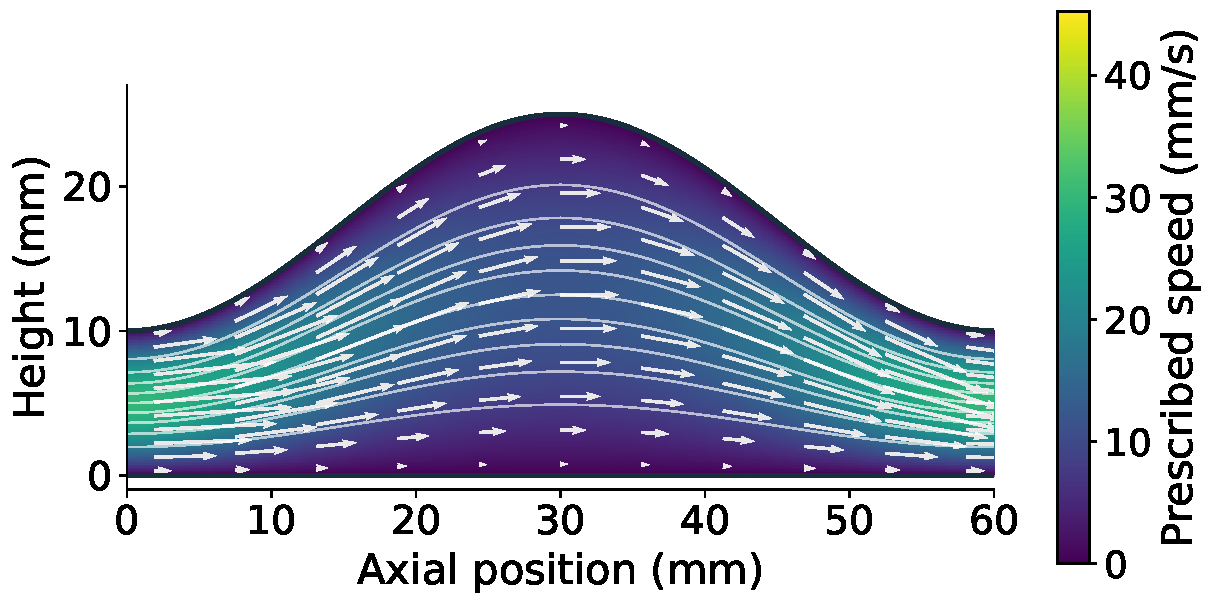
\includegraphics[width=.98\linewidth,height=.69\textheight,keepaspectratio]{presentation-figures/synthetic-chamber-panel-1.pdf}\end{frame}
\renewcommand{\notestarget}{notes.pdf\#note-streamfunction-construction-in-mapped-coordinates}
\begin{frame}[label=slide-the-physical-velocity-panel-2]{B: circulation $\alpha$ =\allowbreak{} 24}
\centering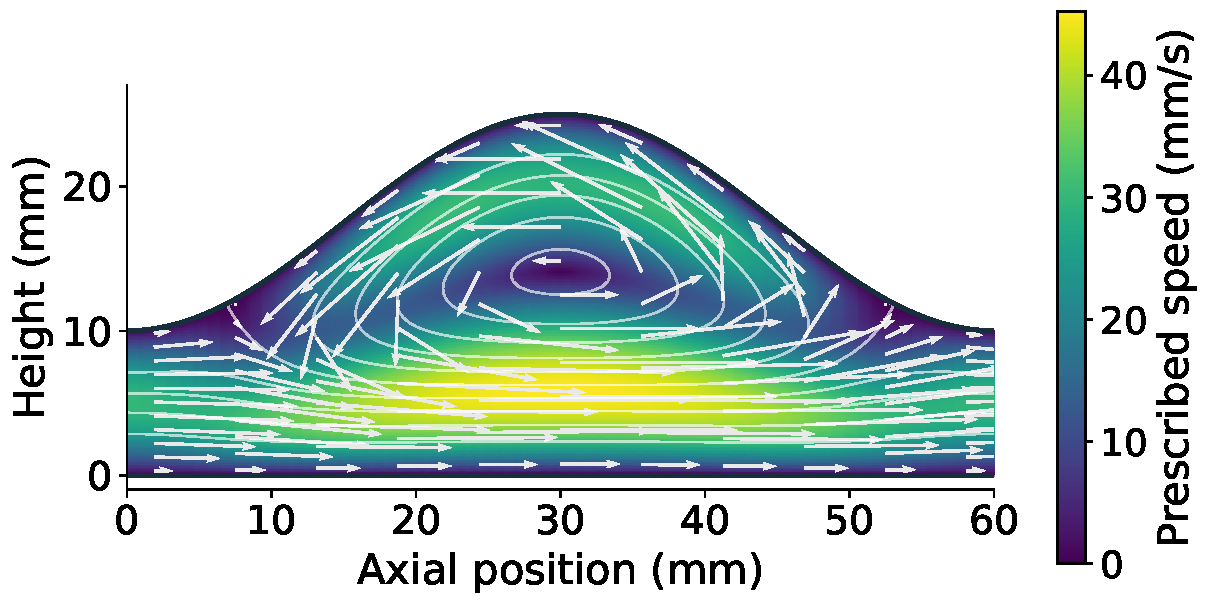
\includegraphics[width=.98\linewidth,height=.69\textheight,keepaspectratio]{presentation-figures/synthetic-chamber-panel-2.pdf}\end{frame}
\renewcommand{\notestarget}{notes.pdf\#note-streamfunction-construction-in-mapped-coordinates}
\begin{frame}[t,fragile,label=slide-the-physical-velocity]{The physical velocity}
\[u=\frac{\psi_\eta}{H},\qquad v=-\psi_x+\frac{\eta H^{\prime}}H\psi_\eta.\]\pause{} Omitting the map term changes the field.
\end{frame}
\renewcommand{\notestarget}{notes.pdf\#note-streamfunction-construction-in-mapped-coordinates}
\begin{frame}[t,fragile,label=slide-cancellation-of-mixed-derivatives]{Cancellation of mixed derivatives}
\[\partial_xu+\partial_yv=\partial_{xy}\psi-\partial_{yx}\psi=0.\]\pause{} Smoothness gives incompressibility. It does not give momentum balance.
\end{frame}
\renewcommand{\notestarget}{notes.pdf\#note-streamfunction-construction-in-mapped-coordinates}
\begin{frame}[t,fragile,label=slide-flux-through-a-cross-section]{Flux through a cross-section}
\[q=\psi(x,H(x))-\psi(x,0),\qquad Q=Wq.\]\pause{} Interior changes can leave this difference unchanged.
\end{frame}
\renewcommand{\notestarget}{notes.pdf\#note-cell-fluxes-and-derivative-reconstruction}
\begin{frame}[t,fragile,label=slide-a-closed-cell-flux-identity]{A closed-cell flux identity}
\[\oint_{\partial K}\boldsymbol u\cdot n\,\mathrm ds=\oint_{\partial K}\mathrm d\psi=0.\]\pause{} Corner values telescope for consistently oriented edge fluxes.
\end{frame}
\renewcommand{\notestarget}{notes.pdf\#note-cell-fluxes-and-derivative-reconstruction}
\begin{frame}[label=slide-sampled-derivatives-form-a-different-calculation-panel-1]{Derivative refinement}
\centering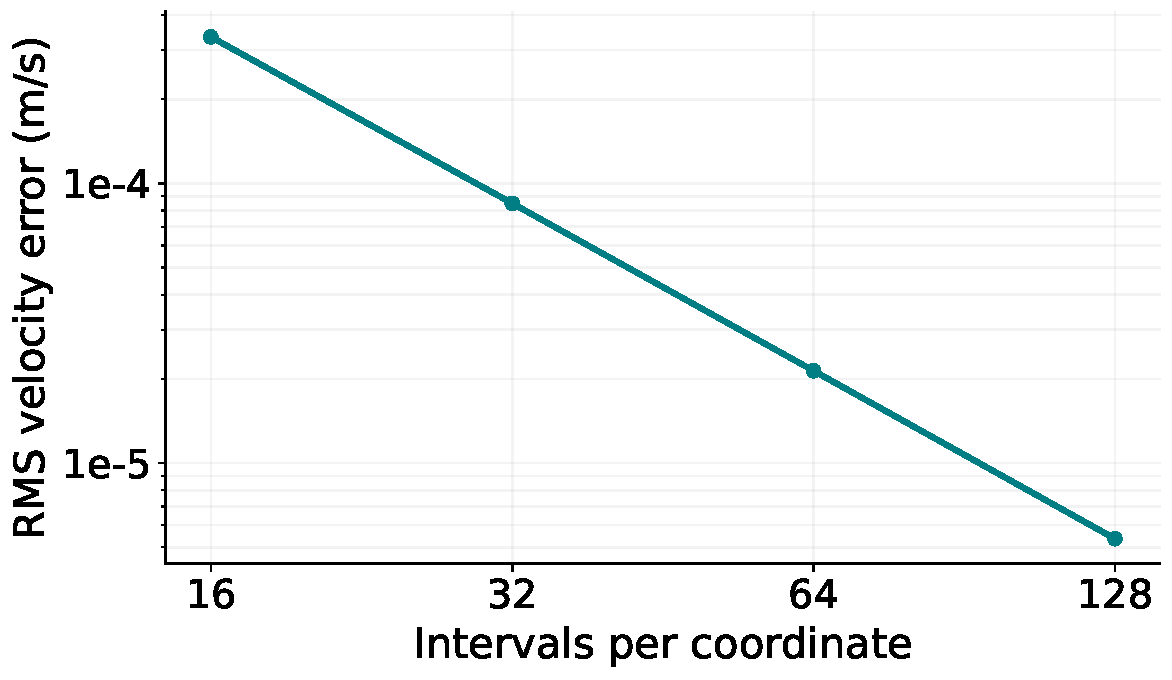
\includegraphics[width=.98\linewidth,height=.69\textheight,keepaspectratio]{presentation-figures/chamber-verification-panel-1.pdf}\end{frame}
\renewcommand{\notestarget}{notes.pdf\#note-cell-fluxes-and-derivative-reconstruction}
\begin{frame}[label=slide-sampled-derivatives-form-a-different-calculation-panel-2]{Input sensitivity}
\centering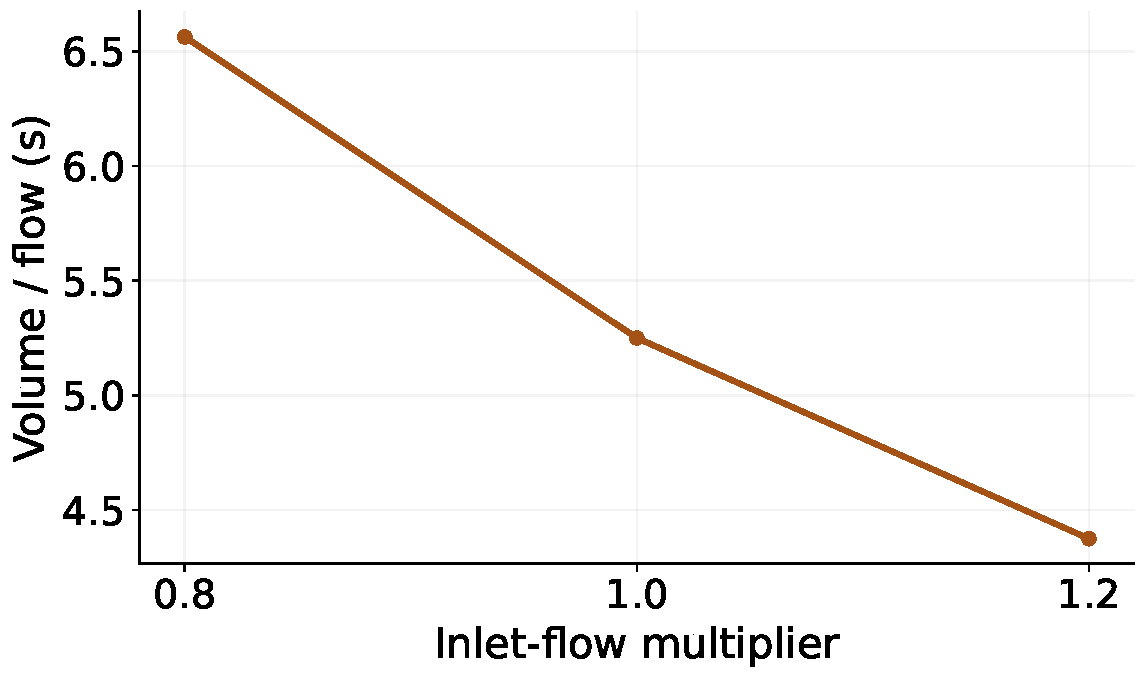
\includegraphics[width=.98\linewidth,height=.69\textheight,keepaspectratio]{presentation-figures/chamber-verification-panel-2.pdf}\end{frame}
\renewcommand{\notestarget}{notes.pdf\#note-cell-fluxes-and-derivative-reconstruction}
\begin{frame}[t,fragile,label=slide-sampled-derivatives-form-a-different-calculation]{Sampled derivatives form a different calculation}
\[\nabla\cdot u=u_x|_\eta-\frac{\eta H^{\prime}}H u_\eta+\frac1H v_\eta.\]\pause{} Derivative reconstruction has a mesh error even when corner fluxes cancel exactly.
\end{frame}
\renewcommand{\notestarget}{notes.pdf\#note-integrated-observations-and-interior-nonuniqueness}
\begin{frame}[t,fragile,label=slide-the-nullspace-of-a-port-flow-observation]{The nullspace of a port-flow observation}
\[\psi_\alpha=\psi_0+\alpha\chi,\qquad\mathcal Q(\chi)=0.\]\pause{} Then $\mathcal Q(\psi_\alpha)=q$ for every $\alpha$, although the interior velocities differ.

Here $\mathcal Q(\psi)=\psi(x,H(x))-\psi(x,0)$ is flux per unit width; total flow is $Q=W\mathcal Q(\psi)$.
\end{frame}
\renewcommand{\notestarget}{notes.pdf\#note-sensitivity-of-a-bulk-turnover-scale}
\begin{frame}[t,fragile,label=slide-a-bulk-turnover-scale]{A bulk turnover scale}
\[T_{\rm bulk}=\frac VQ=\frac{21\ \mathrm{mL}}{4\ \mathrm{mL/s}}=5.25\ \mathrm s.\]\pause{} This ratio does not assign a residence time to each particle.
\end{frame}
\renewcommand{\notestarget}{notes.pdf\#note-sensitivity-of-a-bulk-turnover-scale}
\begin{frame}[t,fragile,label=slide-boundary-input-sensitivity]{Boundary-input sensitivity}
\[T(0.8Q)=6.5625\ \mathrm s,\qquad T(1.2Q)=4.375\ \mathrm s.\]\pause{} Refining numerical derivatives cannot remove uncertainty in the prescribed input.
\end{frame}
\renewcommand{\notestarget}{notes.pdf\#note-prescribed-kinematics-and-the-unresolved-momentum-balance}
\begin{frame}[t,fragile,label=slide-the-missing-dynamical-constraint]{The missing dynamical constraint}
A viscous-flow calculation also requires pressure, acceleration, stress and compatible forcing or boundary data.\pause{} The streamfunction fixture supplies exact kinematics, not a solved atrial CFD model.
\end{frame}
\end{document}
